\documentclass[12pt, twoside, a4paper]{report}
\usepackage{amsmath}
\usepackage{ragged2e}
\usepackage{fancyhdr}
\usepackage{graphicx}

\title{CS2810 - Group Report}
\author{Marcus Messer, Toby Such, Roger Milroy, Andrew Nicolalde,\\
Jonathan Lewin, Robin Chabouk, Johan Rehman}
\date{\today}

\begin{document}
\maketitle
\pagestyle{fancy}
\fancyhf{}
\lhead{CS2810 - Group Report}
\rfoot{Page \thepage}

\section*{Description Of Components}
\subsection*{Views}
\subsubsection*{Customer}
\paragraph{Start Order Page}

\paragraph{Menu Page}

\paragraph{Basket Page}

\subsubsection*{Waiter}
\paragraph{Orders Page}

\paragraph{Edit Order View}

\subsubsection*{Kitchen}

\subsubsection*{Manager}
\paragraph{Manager Home Page}

\paragraph{Edit Menu Page}

\paragraph{Assign Tables Page}

\paragraph{Employee Page}

\subsection*{Server}

\subsection*{Database}
\begin{figure}[h]
  \centering
  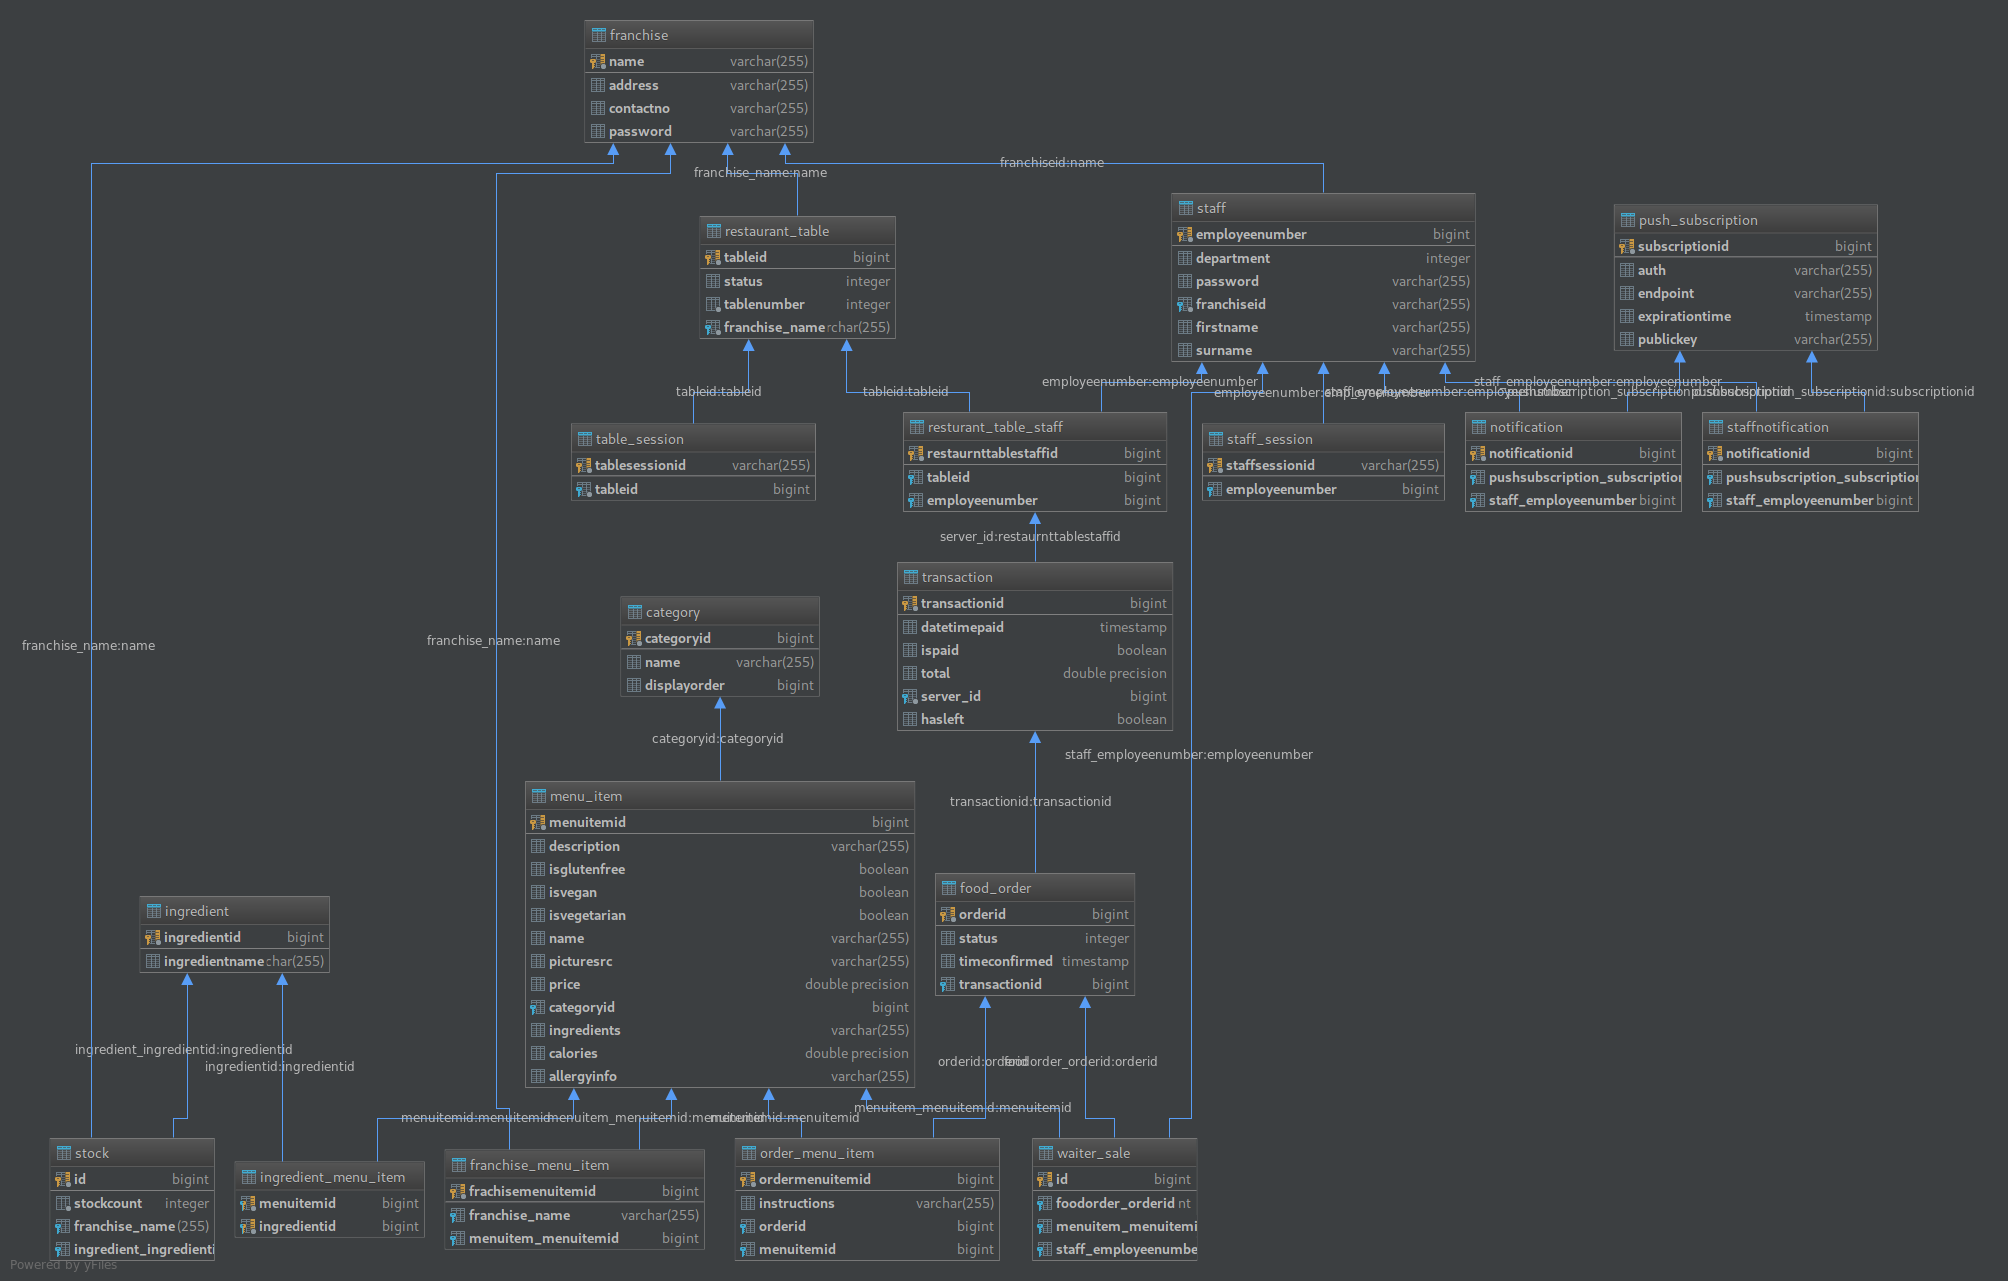
\includegraphics[width=15cm]{database.png}
  \caption{Generated by DataGrip}
  \label{fig:data}
\end{figure}

We have a database with 19 related tables, see Figure \ref{fig:data}. 

The database stores everything including the staff, the menu and the customers orders. 
It also stores the logged in sessions and the data needed for push notifications.
The database was designed to allow the user to start multiple orders and store them onto a transaction that allows the users to pay for all there orders in one go.

\section*{Description Of Packages}
\subsection*{PACKAGE}
\subsubsection*{Implemented Components}
\subsubsection*{Functionality}

\section*{User Stories}
\subsection*{Fully Completed}
These are the completed user stories.
\subsubsection*{Customer Stories}
\begin{itemize}
  \item Electronic Payment
  \item View Menu
  \item Ordering
  \item Menu Filtering
  \item Calling The Waiter
  \item Allergies And Calories
  \item Food Pictures
  \item Order Tracking
  \item Intuitive Ordering
\end{itemize}

\subsubsection*{Waiter Stories}
\begin{itemize}
  \item Notification For Delivery
  \item Cancel Order
  \item Order Times
  \item Payment Information
  \item Order Confirmation
  \item Table Assignment
  \item Mark Order as Delivered
  \item Client Needs Help
  \item Add Extra Sales
  \item Change Status Of An Order
\end{itemize}

\subsubsection*{Kitchen Stories}
\begin{itemize}
  \item Notify Waiters
  \item Confirmed Customer Order
  \item Order Times
\end{itemize}

\subsubsection*{Manager Stories}
\begin{itemize}
  \item Assign Tables
  \item Set Prices
\end{itemize}

\subsection*{Nearly Completed}
These stores are worthy of a mention as they are very nearly finished.

\subsubsection*{Manager Stories}
\begin{itemize}
  \item Adjust Menu:
    The only feature left uncompleted is uploading an image to the new menu item or when editing a menu item.
  \item Add Staff:
    The only feature left is the ability to reset a users password.
\end{itemize}

\section*{Statement of Relative Contribution}
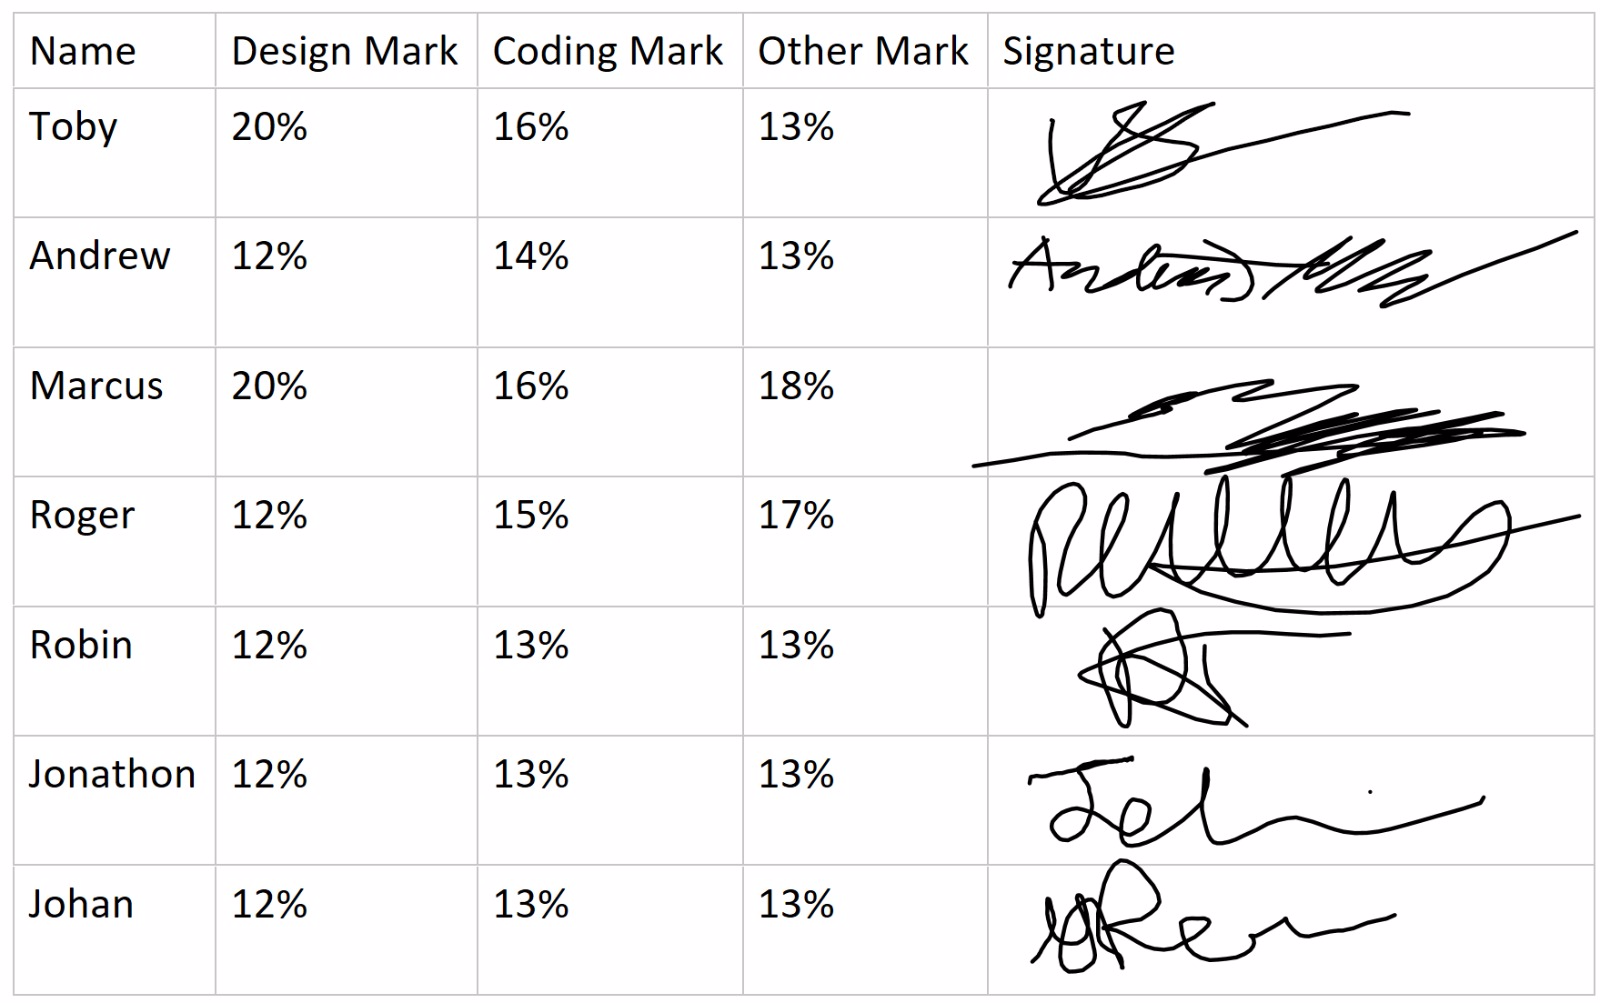
\includegraphics[width=15cm]{StateOfCont.png}

\end{document}
